%!TEX root = ..\ms-thesis.tex
\chapter{Literature Review} \label{ch:literature-review}

\section{Weldability Evaluation} \label{sec:weldability-evaluation}

\subsection{Characteristics of a Weldability Test}

\subsection{The Hot Ductility Test}

\subsubsection{Hot Ductility Evaluation Criteria}
In one of their early studies utilizing the Gleeble hot ductility test, Nippes et al. \cite{nippes_further_1957} classified the observed hot ductility responses of the various alloys into several categories, based on the shapes of the hot ductility curves: Classes H1 or H2 for the on-heating behavior and Classes C1, C2, or C3 for the on-cooling behavior. Schematic hot ductility curves illustrating the characteristics of each behavior class are shown in Figure \ref{fig:nippes-criteria} and a brief text description for each is provided in Table \ref{tab:nippes-classification}. Of the two on-heating behavior categories, Class H2 (Figure \ref{fig:nippes-criteria}b) behavior was identified as being intrinsically sensitive to hot cracking. However, material exhibiting Class H1 behavior (Figure \ref{fig:nippes-criteria}a) was not considered in and of itself indicative of a propensity for hot cracking and thus required the evaluation of on-cooling results to determine the material's susceptibility. With regard to the on-cooling categories, materials exhibiting Class C1 (Figure \ref{fig:nippes-criteria}c) behavior were considered not sensitive to hot cracking. Class C2 and Class C3 behaviors (Figure \ref{fig:nippes-criteria}d,e) were associated with a higher sensitivity to hot cracking, with Class C3 behavior indicating the greatest sensitivity. In particular, Nippes et al. found that those materials in the study which were known to exhibit hot cracking, based on field experience, exhibited Class C3 behavior with on-cooling ductility of 40\% or less of the on-heating ductility. Thus, using the Nippes classification system, in most cases a material's on-cooling ductility response will be the major indicating factor regarding its hot cracking susceptibility. Materials exhibiting Class C3 on-cooling behavior with a low recovery of on-cooling ductility (0-40\% of on-heating ductility) can be identified as showing the greatest susceptibility to hot cracking.

\begin{figure}[h]
\centering
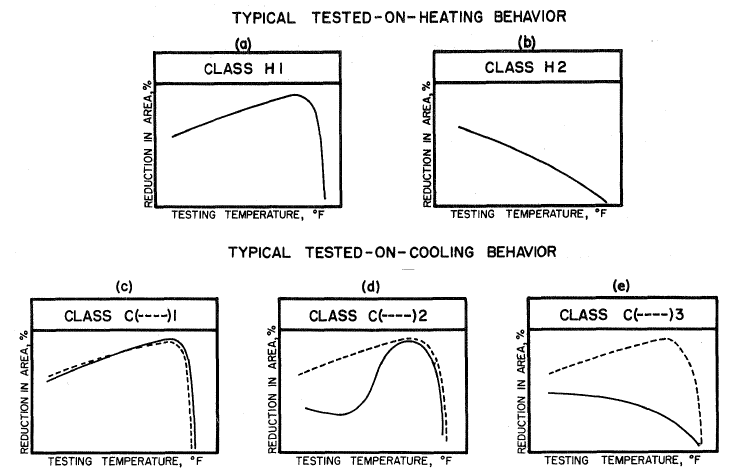
\includegraphics[width=6in]{figures/nippes-criteria.png}
\caption{Classification of Hot Ductility Behavior for On-heating and On-Cooling Tests; in (c), (d), and (e), the solid line is the on-cooling curve and the dashed line is the on-heating curve.  From \citet[Fig.~66]{nippes_further_1957}.}
\label{fig:nippes-criteria}
\end{figure}

\begin{table}[h]
\caption{Classification of on-heating and on-cooling hot ductility responses based on the work of \citet{nippes_further_1957}. Schematic curves for each behavior class are depicted in Figure \ref{fig:nippes-criteria}.}
\begin{tabular}{ lp{4in} }
\toprule
\textbf{Classification} & \textbf{Description} \\
\midrule
On-Heating Class H1 & On-heating ductility generally increases as temperature increases, followed by a sudden loss of ductility over a relatively narrow range as the temperature increases further toward the melting point. (Figure \ref{fig:nippes-criteria}a) \\
On-Heating Class H2 & On-heating ductility shows a gradual decrease over a wide temperature range as the temperature increases toward the melting point. (Figure 3b) \\
& \\
On-Cooling Class C1 & On-cooling ductility is the essentially same as on-heating ductility at all test temperatures. (Figure \ref{fig:nippes-criteria}c) \\
On-Cooling Class C2 & On-cooling ductility is the same as on-heating ductility at test temperatures of 2100°F or above, but is significantly lower at test temperatures in the range of 1800--2000°F. (Figure \ref{fig:nippes-criteria}d) \\
On-Cooling Class C3 & On-cooling ductility is lower than on-heating ductility at all test temperatures; severity of ductility decrease may change with on-cooling test temperature or with the peak temperature utilized for the on-cooling thermal cycle. (Figure \ref{fig:nippes-criteria}e) \\
\bottomrule
\end{tabular}
\label{tab:nippes-classification}
\end{table}


Further investigation of hot ductility test criteria was undertaken in a review by \citet{yeniscavich_correlation_1970}. One of the criteria reviewed, attributed to Nippes, was the ductility recovery rate (DRR). According to this criteria, crack-resistant materials show a rapid recovery of on-cooling ductility after exposure to the HAZ peak temperature, while the on-cooling ductility for crack-sensitive materials recovers slowly and remains low even at test temperatures well below the peak temperature. Schematic curves illustrating the DRR for crack-resistant and crack-sensitive materials are shown in Figure \ref{fig:drr-schematic}. Numerically, the DRR is determined by taking the ratio of the on-cooling ductility to the on-heating ductility at a specified temperature, typically the rapid-ductility-decrease temperature on the on-heating curve (the point on the curve immediately prior to the sudden drop in ductility).

\begin{figure}
\centering
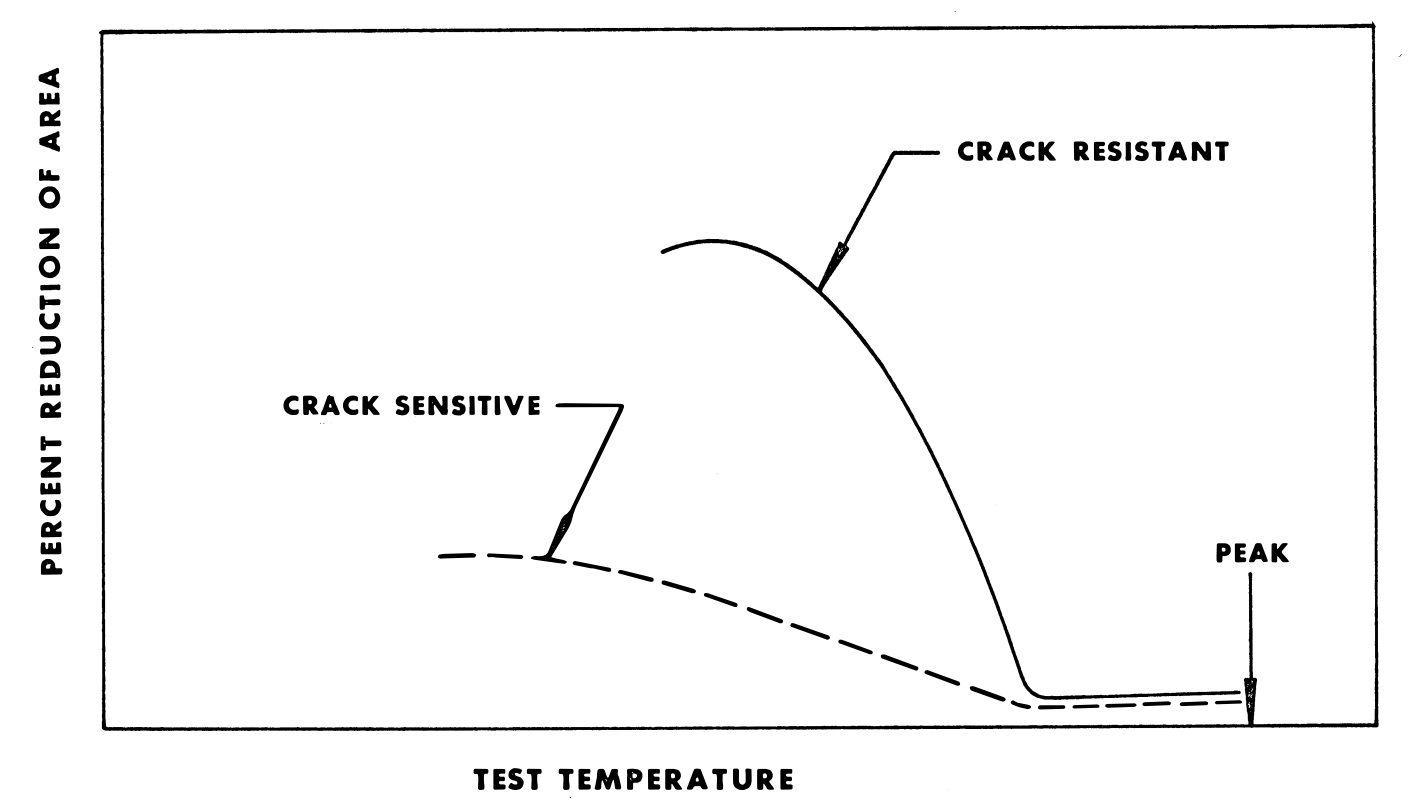
\includegraphics[width=6in]{figures/yeniscavich-drr.png}
\caption{Schematic curves illustrating the on-cooling ductility recovery rate (DRR) criteria for crack-resistant and crack-sensitive materials.  From \citet[Fig.~2]{yeniscavich_correlation_1970}}
\label{fig:drr-schematic}
\end{figure}

Yeniscavich also proposed the \nomenclature{ZDR}{Zero ductility temperature range} zero ductility temperature range (ZDR) as an improved indicator of propensity for hot cracking. The ZDR phenomenon corresponds to a finite temperature increment below the ZDT in which the on-cooling ductility remains zero, i.e. the ductility does not immediately increase once the on-cooling test temperature is below the ZDT. The physical significance of the ZDR is related to the fact that the HAZ must possess sufficient ductility to withstand the thermal strains imposed during welding, otherwise cracking will occur. Since the magnitude of these strains is small over the length scale of an HAZ, the HAZ ductility must be on the order of zero for hot cracking to be of concern. Thus, alloys which show a large ZDR (zero ductility over a wide on-cooling temperature range) are considered more vulnerable to hot cracking than alloys which show a narrow ZDR (see Figure \ref{fig:zdr-schematic}).

\begin{figure}
\centering
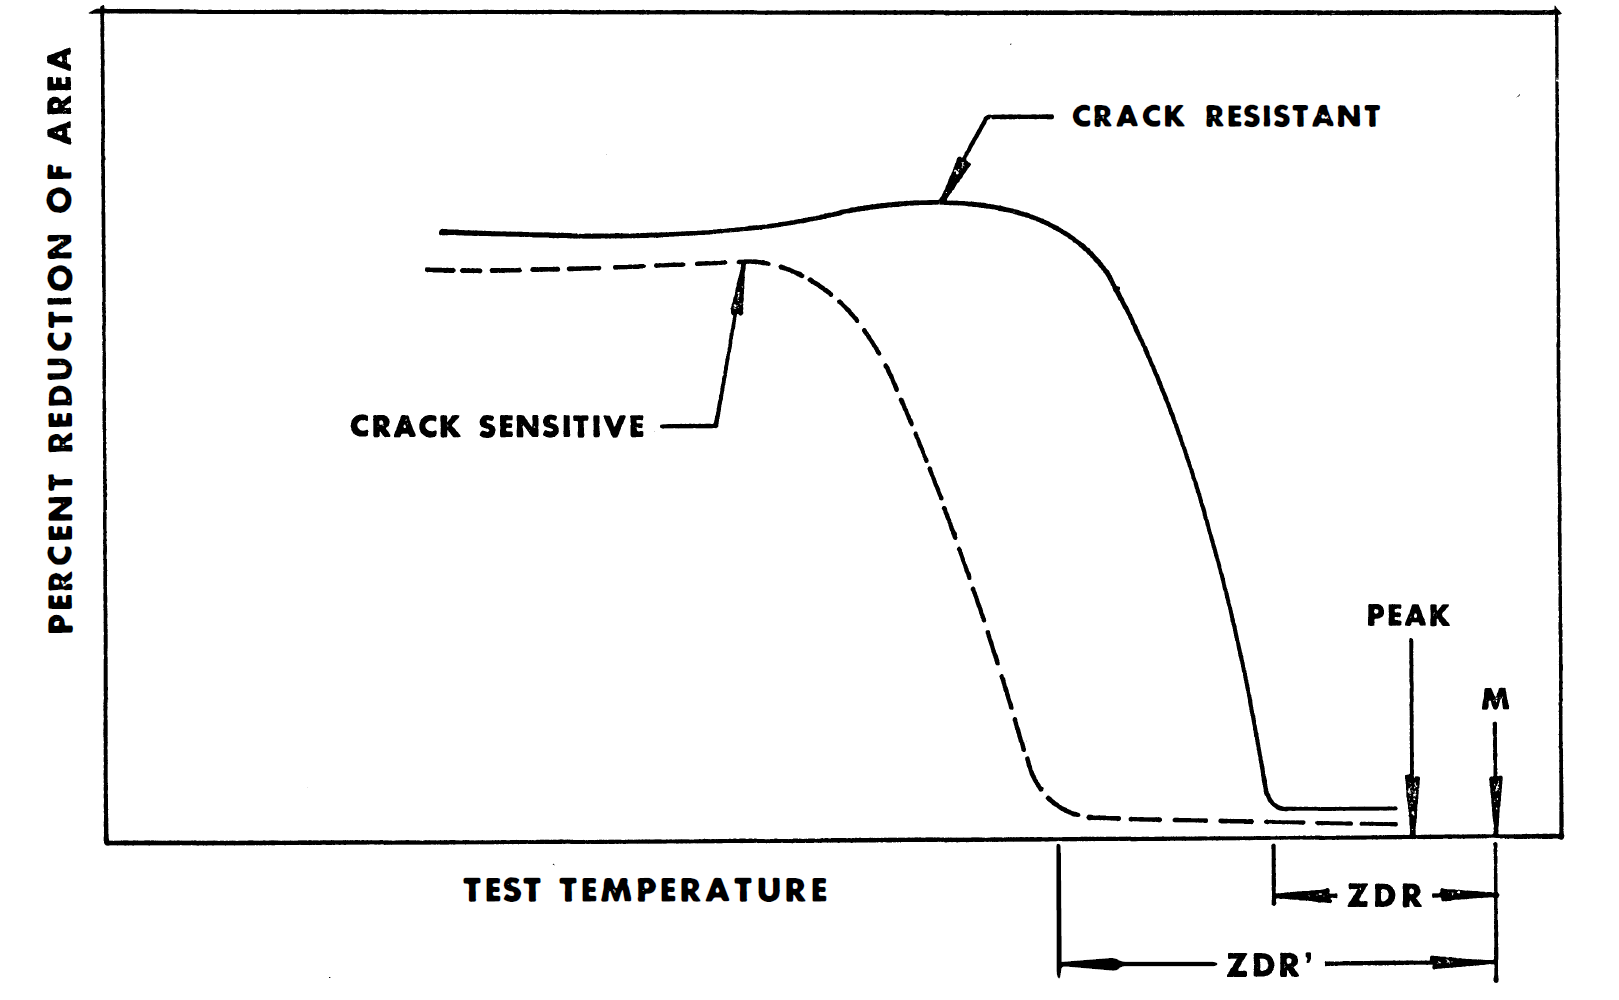
\includegraphics[width=6in]{figures/zdr-schematic.png}
\caption{Schematic of Hot Ductility Curves Illustrating Different On-Cooling Behaviors According to the Zero Ductility Range Criteria: Crack-Sensitive (ZDR') and Crack-Resistant (ZDR).  From \citet[Fig.~4]{yeniscavich_correlation_1970}}
\label{fig:zdr-schematic}
\end{figure}


